\documentclass[11pt]{thyv}

\usepackage[utf8]{inputenc}
\RequirePackage[T1]{fontenc}
\usepackage{xcolor}
\usepackage{tikz}
\usepackage{graphicx}
\usepackage{amsmath}
\usepackage{marvosym}
\usepackage{relsize}
\usepackage{doi}
\usepackage{url}
\usepackage{hyperref}

    \definecolor{thyFirst}{RGB}{132,70,132}
    \definecolor{thySecond}{RGB}{70,70,132}
    \definecolor{thyThird}{RGB}{170,60,60}
    \definecolor{thyGrey}{RGB}{100,100,100}

\begin{document}

	\begin{tikzpicture}[remember picture,overlay]
   		\node [rectangle, anchor=north, minimum width=6cm, minimum height=\paperheight+1cm] (box) at (-5cm,1.5cm){};
	\end{tikzpicture}

	%------------------------------------------------

	\begin{textblock}{5}(0.5, 0)

		%------------------------------------------------

		
			\begin{center}
				\begin{tikzpicture}[x=\imagescale,y=-\imagescale]
					\clip (300, 300) circle (300);
					\draw[line width=2pt] (300, 300) circle (300);
					\node[anchor=north west, inner sep=0pt, outer sep=0pt] at (0,0) {
						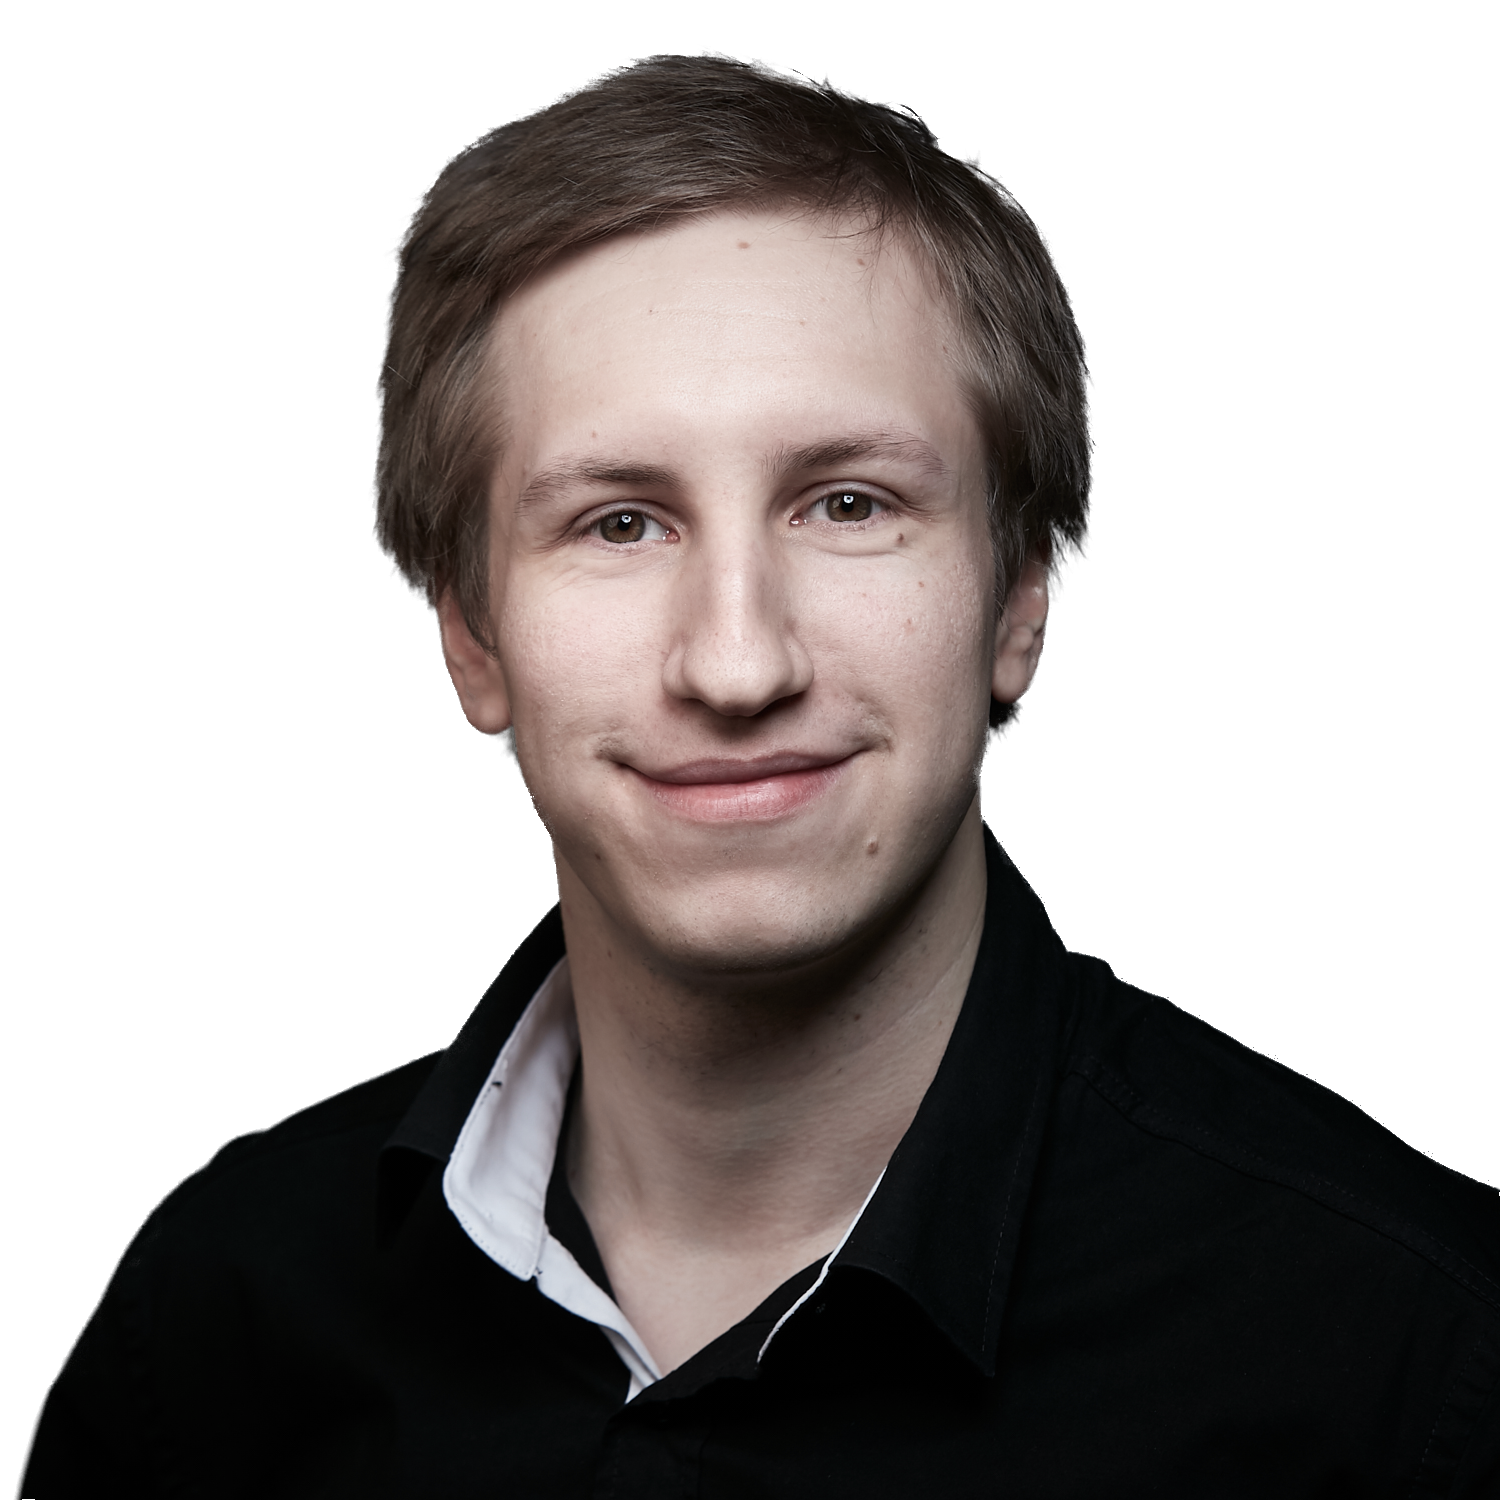
\includegraphics[width=\imagewidth]{max0.6.png}
					};
				\end{tikzpicture}
			\end{center}
		

		%------------------------------------------------


		{\Large Max-Jonathan Luckow}

		%------------------------------------------------

		{Computer Science Student}

		\strut

	\begin{thyV}{2010}{2024}{21}{0.6\linewidth}
		\thyVent{high-school\\ diploma} 				{6/2010}
		\thyVent{Publication} 							{1/2020}
		\thyVent{B.Sc.\\Thesis} 						{3/2017}
		\thyVent{\\ M.Sc.Thesis} 						{3/2023}
		
		\thyVentEdu{Energy and\\Process Engineering} 	{4/2011}{9/2013} 	{}
		\thyVentEdu{Bachelor of Science \\Computer Science} 			{10/2013}{3/2017} 	{16.625/2014} 
		\thyVentEdu{Master of Science \\ Computer Science} 			{4/2017}{3/2023} 	{7.25/2020}

		\thyVentWork{Technical\\Accountant} 			{9/2020}{4/2022} 	{}
		\thyVentWork{Web Developer} 					{3/2018}{4/2018} 	{}
		\thyVentWork{Technical Specialist} 				{6/2017}{11/2017} 	{9.25/2017}
		\thyVentWork{Self-employed} 					{1/2014}{5/2017} 	{22.875/2014}

		\thyVentWork{Assistant in \\ surgical ward} 	{8/2010}{1/2011} 	{12.25/2010}
	\end{thyV}

		\thyLegend{Experience}{1.8cm}{thySecond} \thyLegend{Education}{1.8cm}{thyFirst} \thyLegend{Events}{1.1cm}{thyThird}
		%\parbox{2cm}{{\rule{1.5cm}{3pt}}\\Education}
		%\parbox{2cm}{{\rule{1.5cm}{3pt}}\\Experience}
		%\parbox{2cm}{{\rule{1.5cm}{3pt}}\\Experience}
		
		\begin{tabular}{lll}
		{\rule{1.5cm}{3pt}} & {\rule{1.5cm}{3pt}} & {\rule{1.5cm}{3pt}} \\
		Education & Experience & Events
		\end{tabular}

	\end{textblock}

	\begin{mdframed}

		\begin{minipage}[t]{0.50\textwidth} % 27.5% of the page width for the first row of icons
			\vspace{-\baselineskip} % Required for vertically aligning minipages

			\icon{Cross}{12}{30. Dezember 1990}\\
			\icon{Phone}{12}{+49 163 222 99 64}\\
				
		\end{minipage}
		\begin{minipage}[t]{0.50\textwidth} 
			\vspace{-\baselineskip} % Required for vertically aligning minipages
			
			\icon{At}{12}{\href{mailto:max@luckow.ch}{max@luckow.ch}}\\
			\icon{Github}{12}{\href{https://github.com/Carlisle96}{github.com/Carlisle96}}\\
		\end{minipage}


		\thyVsection{Publication}{thyThird}
			M. J. Luckow and T. Fluschnik. \textbf{``\href{https://doi.org/10.1016/j.ipl.2019.105913}{On the Computational Complexity of Length- and Neighborhood-Constrained Path Problems}''}. In: \textit{Information Processing Letters.} Vol. 156 (2020). \hfill \textcolor{thyGrey}{1/2020} %\texttt{\doi{10.1016/j.ipl.2019.105913}}
		
		\thyVsection{Technical Expertise}{thyBlack}
			C/\Cplusplus, Java, Python \hfill \ThreeOfFour \\
			Latex \hfill \ThreeOfFour \\
			Haskell \hfill \OneOfFour \\
			Linux \hfill \TwoOfFour \\
			Solidity \hfill \TwoOfFour \\
			Javascript, Vue.js, Node.js, SQL \hfill \TwoOfFour \\
			%\vfill\null
			%\columnbreak
			Datev Uno \hfill \FourOfFour

		\thyVsection{Work Experience}{thySecond}
			\thyntry{Technical Acountant}{Agilo-Services GmbH}{9/2020 -- present}
			{Analysis, optimization and automation of the accounting system}
			{Datev Uno \slashsep Haskell}

			\thyntry{Web Developer}{Trado GmbH}{3/2018 -- 4/2018}
			{Programming and maintenance of the internal administrative software}
			{Javascript \slashsep Node.js \slashsep Vue.js \slashsep SQL}

			\thyntryLast{Technical Specialist}{Envion AG}{6/2017 -- 11/2017}
					{Analysis of Cryptocurrency market
			    	\\ Devolopment of the first mining operations prototype
			    	\\ Supervision of the production of the first large scale mining operation}
			    	{Linux \slashsep Solidity}

			%\thyntrySmall{Self-employed}{}{1/2014 -- 5/2017}
			%{IT administration, development and project support}

			%\thyntrySmall{Assistant in surgical ward}{Hospital Waldfriede Berlin}{08/2010 -- 01/2011}
			%{Community service}

		\thyVsection{Education}{thyFirst}

			\thyntry{Master of Science. Computer Science}{Technical University of Berlin}{4/2017 -- \textit{3/2013}}{Specialisation in cognitive systems}{Java \slashsep Python \slashsep Solidity}

			\thyntryLast{Bachelor of Science. Computer Science}{Technical University of Berlin}{4/2017 -- \textit{3/2013}}{Area of study in foundations of computing with the thesis on algorithms and complexity}{C/\Cplusplus \slashsep Java \slashsep Python \slashsep SQL \slashsep Latex}{}

			%\thyntrySmall{Energy and Process Engineering}{Technical University of Berlin}{4/2011 -- 9/2013}{}

			%\thyntrySmall{High-school diploma}{Arndt Gynasium Dahlem}{8/2003 -- 6/2010}{}

		\thyVsection{Language Expertise}{thyBlack}
			German: Native speaker \\
			English: Advanced \\
			Latin: Latinum

		\vspace{-25pt}

		\begin{textblock}{5}(17.5, 27.7)
		
\includegraphics[width=3cm]{signature2.png}
		\end{textblock}
	\end{mdframed}




\end{document}